\documentclass[11pt,a4paper]{article}

\usepackage[margin=2.5cm]{geometry}
\usepackage[T1]{fontenc}
\usepackage{lmodern}
\usepackage{microtype}
\usepackage{graphicx}
\usepackage{booktabs}
\usepackage{tabularx}
\usepackage{xltabular}
\usepackage{enumitem}
\usepackage{xcolor}
\usepackage{caption}
\usepackage{listings}
\usepackage{tikz}
\usetikzlibrary{positioning,arrows.meta,fit,backgrounds}
\usepackage{pgfplots}
\pgfplotsset{compat=1.18}
\usepackage{placeins}
\usepackage[hidelinks]{hyperref}
\usepackage[nameinlink,capitalise]{cleveref}

\emergencystretch=2em
% keep figures and tables inside the subsection that introduces them
\let\oldsubsection\subsection
\renewcommand{\subsection}{\FloatBarrier\oldsubsection}
\setlist{itemsep=2pt,topsep=4pt}
\setlength{\parskip}{4pt}
\captionsetup{font=small,labelfont=bf}

\definecolor{wf}{HTML}{1F5FA8}    % our workflow (A)
\definecolor{rag}{HTML}{8A94A3}   % simple RAG (C)
\definecolor{cb}{HTML}{D08A2E}    % closed book (N)
\definecolor{llmbox}{HTML}{FBE7C6}

\lstset{basicstyle=\ttfamily\small,breaklines=true,columns=fullflexible,
        frame=single,rulecolor=\color{gray!40},backgroundcolor=\color{gray!6}}

\newcommand{\code}[1]{\texttt{#1}}

% Placeholder for a screenshot that will be added later:
%   \screenshot{what to capture}{caption}{label}
% Replace it with \includegraphics[width=\linewidth]{figures/<file>} once the image exists.
\newcommand{\screenshot}[3]{%
  \begin{figure}[ht]\centering
  \fbox{\parbox[c][35mm][c]{0.8\linewidth}{\centering\small\color{gray}%
    \textbf{Screenshot to add:}\\[2pt] #1}}
  \caption{#2}\label{#3}
  \end{figure}}

\begin{document}

\begin{titlepage}
\centering
\vspace*{2cm}
{\LARGE\bfseries A Financial Question-Answering Agent\\[4pt] with Cited Answers from SEC Filings\par}
\vspace{1cm}
{\large COMP4651 Cloud Computing and Big Data Systems\par}
{\large Project report\par}
\vspace{1.5cm}
\begin{tabular}{lp{9.5cm}}
Project category: & Deep project (D3) \\
Group number:     & Group 10 \\[6pt]
Group members:    & Kaan Bayraktar \\
                  & Anton Hansen \\
                  & Simon Strandgaard \\[6pt]
Word count:       & about 4,700 (Introduction to Conclusion, excluding tables, figures, captions and references) \\
GitHub:           & \small\url{https://github.com/Cloud-Computing-group-10/financial-agent-project} \\
                  & (branch \code{feature/cloud-app}) \\
\end{tabular}
\vfill
{\large 1 December 2026\par}
\end{titlepage}


\tableofcontents
\clearpage

\section{Introduction}

\subsection{Background and motivation}

Every US public company must publish its financial results. Each quarter it files a report called a
10-Q with the Securities and Exchange Commission (SEC), and each year a longer annual report, the
10-K. These filings answer questions such as ``What were 3M's net sales in the second quarter of
2023?'' or ``Why did Honeywell's sales increase?''. They are free to download from the SEC's EDGAR
website~\cite{sec-edgar}, but they are long: a single 10-Q often has 50 pages, and more than 140,000
10-Qs have been filed since 2019.

Large language models (LLMs) such as ChatGPT or Claude can answer such questions in fluent text, but
they make two kinds of mistakes that matter in finance. They may state a number from memory that is
wrong or out of date, and they often get arithmetic wrong even when the correct figures are in front
of them~\cite{financebench,finqa}. A wrong number given with confidence is worse than no answer.

This project builds a question-answering system for company filings that \emph{cites the source of
every number and every reason}, so that a reader can check each claim. The central idea is to give
the LLM as little responsibility as possible: it only interprets the question and phrases the final
answer, while ordinary code finds the figures, computes changes and checks the citations. To answer
questions about any company, the system needs the data of every filer, so the project also has a
cloud and big data side: tens of gigabytes of SEC data are processed with Spark on AWS.

\subsection{Literature review}

\paragraph{Financial question answering.} Questions about financial reports mix text, tables and
arithmetic. The FinQA~\cite{finqa} and TAT-QA~\cite{tatqa} benchmarks pair questions with a table and
some text from an annual report; both found that models are much better at finding the right numbers
than at computing with them. FinanceBench~\cite{financebench} is closer to real use: 150 questions
written by financial analysts about real 10-K and 10-Q filings. Its authors found that a standard
LLM pipeline answered most of them incorrectly or not at all. We use it as an external test set.

\paragraph{Retrieval-augmented generation (RAG).} RAG~\cite{rag} is the standard way to let an LLM
answer from documents it was not trained on: a search step selects the most relevant passages and
gives them to the LLM together with the question. Search can be \emph{lexical}, such as
BM25~\cite{bm25}, which scores passages by the words they share with the question, or
\emph{semantic}, which turns texts into vectors (embeddings) with a model such as
MiniLM~\cite{minilm,sbert} and compares how similar they are. Reciprocal rank fusion~\cite{rrf}
combines the two rankings. RAG does not stop the LLM from adding facts that are not in the
passages~\cite{hallucination}, and it does not help with arithmetic. Program-of-thought
prompting~\cite{pot} moves arithmetic out of the LLM into code; we go one step further and take the
most common numbers directly from structured data.

\paragraph{Big data and small models.} Apache Spark~\cite{spark} processes large datasets in
parallel, on one machine or on a cluster. Postgres with the pgvector extension~\cite{pgvector} stores
embeddings next to ordinary tables, so figures, filings and passages can live in one database. Small
open models such as Qwen2.5~\cite{qwen25} run on a laptop at no cost per question but are less
reliable. Whether a careful design makes such models useful is one of our research questions.

\subsection{Objectives}

\begin{enumerate}
  \item Build a question-answering workflow over SEC filings in which code, not the LLM, finds and
        computes every number, and every claim cites a filing, a statement line or a passage.
  \item Build a data pipeline on AWS that uses Spark to load the figures and the 10-Q text of every
        SEC filer since 2019 into one database.
  \item Compare the workflow with simpler systems on our own question set and on FinanceBench, using
        a hosted LLM (Claude Haiku 5.5) and small local LLMs (Qwen2.5 with 3 and 7 billion
        parameters).
  \item Measure the cloud side: time per step, throughput, Spark scaling and the time needed to add
        new filings.
\end{enumerate}

\section{Methodology: design}

\subsection{Scope and data sources}

The system answers questions about the quarterly results of US public companies. It uses three
public datasets from the SEC and one benchmark (\cref{tab:data}).

\begin{table}[ht]
\centering\small
\begin{tabularx}{\linewidth}{lXl}
\toprule
Source & What we use & Size \\
\midrule
\code{companyfacts.zip} & XBRL figures of every filer; we keep 10 metrics per 10-Q & 1.4 GB, 20,609 files \\
\code{submissions.zip} & List of filings per company, to find each 10-Q document & 1.5 GB \\
10-Q documents (EDGAR) & Text passages from the MD\&A section, for ``why'' questions & 140,226 filings \\
FinanceBench~\cite{financebench} & 150 questions with analyst answers, 84 PDF filings & 160 MB \\
\bottomrule
\end{tabularx}
\caption{Data sources.}
\label{tab:data}
\end{table}

XBRL (eXtensible Business Reporting Language) is the machine-readable version of the financial
statements that companies file together with each report. Each fact has a tag (for example
\code{Revenues}), a value, a unit and the start and end date of its period. This gives us exact
numbers without parsing tables. We keep ten metrics: revenue, cost of sales, gross profit, SG\&A,
R\&D, operating income, pretax income, net income, diluted EPS and operating cash flow. Reasons
(``why did sales fall?'') are not in XBRL, so they come from the text of the
\emph{Management's Discussion and Analysis} (MD\&A) section of each 10-Q.

\subsection{Answer workflow}

\Cref{fig:workflow} shows the five steps of a question. Only two of them call an LLM (shaded).

\begin{figure}[ht]
\centering
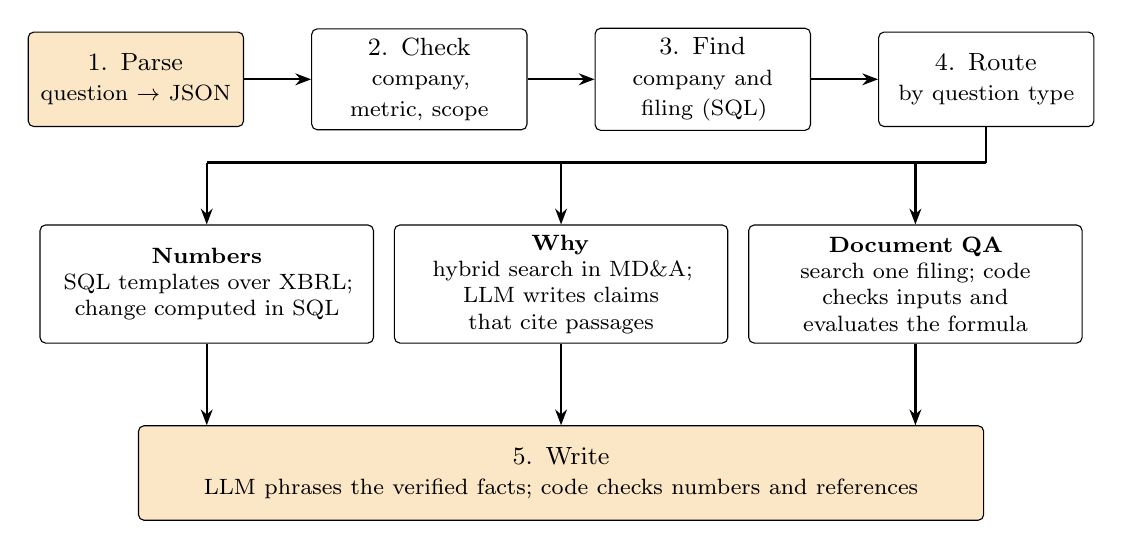
\begin{tikzpicture}[
  box/.style={draw,rounded corners=2pt,align=center,font=\small,minimum height=12mm,text width=25mm},
  llm/.style={box,fill=llmbox},
  path/.style={draw,rounded corners=2pt,align=center,font=\footnotesize,text width=40mm,minimum height=15mm},
  arr/.style={-{Stealth[length=2mm]},thick}]
  \node[llm] (parse) at (0,0)    {1. Parse\\\footnotesize question $\to$ JSON};
  \node[box] (check) at (3.6,0)  {2. Check\\\footnotesize company, metric, scope};
  \node[box] (find)  at (7.2,0)  {3. Find\\\footnotesize company and filing (SQL)};
  \node[box] (route) at (10.8,0) {4. Route\\\footnotesize by question type};
  \node[path] (num) at (0.9,-2.6)  {\textbf{Numbers}\\SQL templates over XBRL; change computed in SQL};
  \node[path] (why) at (5.4,-2.6)  {\textbf{Why}\\hybrid search in MD\&A; LLM writes claims that cite passages};
  \node[path] (doc) at (9.9,-2.6)  {\textbf{Document QA}\\search one filing; code checks inputs and evaluates the formula};
  \node[llm,text width=105mm] (write) at (5.4,-5.0) {5. Write\\\footnotesize LLM phrases the verified facts; code checks numbers and references};
  \draw[arr] (parse)--(check); \draw[arr] (check)--(find); \draw[arr] (find)--(route);
  \draw[thick] (route.south) -- ++(0,-0.45) coordinate (b);
  \draw[thick] (b) -- (b -| num.north);
  \draw[arr] (b -| num.north) -- (num.north);
  \draw[arr] (b -| why.north) -- (why.north);
  \draw[arr] (b -| doc.north) -- (doc.north);
  \draw[arr] (num.south) -- (num.south |- write.north);
  \draw[arr] (why.south) -- (write.north);
  \draw[arr] (doc.south) -- (doc.south |- write.north);
\end{tikzpicture}
\caption{The answer workflow. Shaded steps call the LLM; all other steps are code. The ``why''
path also calls the LLM to write its claims.}
\label{fig:workflow}
\end{figure}

\paragraph{Step 1: parse.} The LLM turns the question into a small JSON object: company (as written
in the question), metric, period (for example \code{Q2 2023}), question type (numeric, explanatory
or both), comparison (year over year, quarter over quarter or none) and search terms. The output must
match a fixed schema.

\paragraph{Step 2: check.} Code then checks the parse. The company must appear in the question
(``ask, don't guess''), the metric must be one of the ten, and a few scope rules always apply: Q4
and full-year numbers are only in the 10-K, and segment numbers are not in our figures. A question
without a ``why'' word is never sent to the explanation path. These checks catch the most common
mistakes of small models.

\paragraph{Step 3: find.} SQL looks up the company (by ticker, a known alias, or a normalised name)
and the filing that covers the period.

\paragraph{Step 4: route.} The question goes to one of three paths.
\begin{itemize}
  \item \textbf{Numbers.} One of the ten metrics for a quarter, or its change. A fixed SQL template
        reads the figure. For a year-over-year change it reads the prior-year column of the
        \emph{same} 10-Q, so restated values are used (for example Johnson \& Johnson after the
        Kenvue spin-off). The change in percent and in dollars is computed in SQL. Each figure cites
        the filing, statement, line label, XBRL tag and period.
  \item \textbf{Why.} Hybrid search (BM25 plus semantic, merged by reciprocal rank fusion) over the
        MD\&A passages of that one filing. If the best match is too weak (cosine similarity below
        0.45), the system declines. Otherwise the LLM writes short claims, each of which must cite a
        retrieved passage by its id; claims that cite an unknown passage are dropped.
  \item \textbf{Document QA.} Everything else: ratios, full years, other line items and text
        questions, as in FinanceBench. The system searches the filing of that period (top 10
        passages). For a calculation the LLM does not give the result. It names each input exactly
        as printed, with the passage it comes from, and a formula. Code checks that each input
        really is printed in that passage and then evaluates the formula (only arithmetic is
        allowed).
\end{itemize}

\paragraph{Step 5: write.} A second LLM call turns the verified facts into a short answer. It gets
only the question and the facts, each with a reference such as
\code{[F1] 3M, net sales, Q2 2023: \$8.325 billion}. Code rejects the answer if it contains a number
that is not in the facts or a reference that does not exist. In that case the system uses a fixed
template answer instead. An example answer:

\begin{lstlisting}
3M's net sales fell year over year in the second quarter of 2023. Net sales were
$8.325 billion in Q2 2023, compared with $8.702 billion in Q2 2022 [F1][F2]. The
computed change is a decrease of 4.3%, or $377 million.
\end{lstlisting}

The design rule is that the user never sees a number that code did not find or compute. A number
question takes two LLM calls (parse, write), a ``why'' question three (parse, claims, write) and a
document QA question two (parse, answer).

\subsection{Database design}

All data lives in one Postgres 16 database with the pgvector extension (\cref{tab:db}).

\begin{table}[ht]
\centering\small
\begin{tabularx}{\linewidth}{lrX}
\toprule
Table & Rows & Contents \\
\midrule
\code{companies}   & 9,695     & CIK, name, main ticker, normalised name for lookups \\
\code{documents}   & 140,520   & One row per filing: form, period, filing date, link, whether text is indexed \\
\code{figures}     & 3,022,763 & Metric, XBRL tag, line label, period, value, unit, derived flag \\
\code{metric\_tags}& 96,950    & Which XBRL tag each company uses for each metric \\
\code{chunks}      & 4,550,888 & Passages of about 180 words, with section, heading and a 384-dimension embedding \\
\bottomrule
\end{tabularx}
\caption{Database tables after the full load.}
\label{tab:db}
\end{table}

Two rules for the figures matter for correctness. A quarter is a fact whose period is about three
months long, labelled from its own end date, and the tag is chosen per filing from an ordered list
of candidates (companies use different tags for ``revenue''). Cash flow is only reported year to
date, so a quarter is computed as the year-to-date value minus the previous year-to-date value and
marked as derived. Every search is filtered to one filing first, so the 4.5 million passages do not
slow a question down.

\subsection{Cloud architecture}

We run everything on one AWS EC2 instance (c7i.8xlarge: 32 vCPUs, 64 GB memory, 250 GB disk,
Ubuntu, region us-east-1) with Docker Compose. The containers are Postgres with pgvector, the
FastAPI service, a Streamlit web page, the Spark jobs and, optionally, Ollama to serve a local LLM
on the CPU. S3 keeps a long-term copy of the raw downloads, the Parquet files and the passages.

We considered an EMR Spark cluster but chose one large machine. The slowest part of the pipeline is
downloading 140,000 documents, and the SEC allows at most 10 requests per second from one user, no
matter how many machines send them. The CPU-heavy part (splitting and embedding text) is spread
over the cores of one machine by Spark just as well as over several machines, without the cost of
starting a cluster. The instance is stopped when it is not used, and the heavy steps are resumable.

\subsection{Baselines}

To show what the workflow adds, we compare it with two simpler systems that use the same LLM.
\begin{itemize}
  \item \textbf{C: simple RAG.} The same passage index and hybrid search over the correct filing,
        top 10 passages, one LLM call that must cite passages. No parsing, routing, SQL, code
        arithmetic or checks.
  \item \textbf{N: closed book.} The LLM gets only the question and must answer from its own
        knowledge, with the same instruction to cite sources or say it does not know. This shows
        whether retrieval is needed at all.
\end{itemize}
We also run \textbf{A0}, our workflow with the template answer instead of the writer, to measure
what the writer LLM adds. A fourth baseline, giving the LLM the whole filing, was built but not run:
it mostly measures how much context a model can take and was the most expensive cell.

\section{Methodology: implementation and deployment}
\label{sec:implementation}

This chapter describes how the design is implemented and deployed. For further details on the setup
and on reproducing every step and experiment, see the file
\href{https://github.com/Cloud-Computing-group-10/financial-agent-project/blob/feature/cloud-app/REPRODUCE.md}{\code{REPRODUCE.md}}
in our source code.

\subsection{Tech stack}

The system is written in Python. \Cref{tab:stack} lists its main components. All LLM calls go through
one module, so the same workflow code runs with the hosted Claude model, with Qwen on a laptop, or
with Qwen served on the cloud machine. One Docker image contains the code, Spark and the embedding
model, and the same Docker Compose file starts the system on a laptop and on AWS. Automated tests
check the rules that decide correctness (periods, metric tags, routing, company lookup, passage
splitting, the formula evaluator and the answer check) and run on every change to the code.

\begin{table}[ht]
\centering\small
\begin{tabularx}{\linewidth}{lX}
\toprule
Component & Used for \\
\midrule
Postgres 16 + pgvector & Figures, filings and passages with their embeddings, in one database \\
PySpark (local mode) & The two batch jobs: XBRL figures to tables, and 10-Q text to embedded passages \\
fastembed (MiniLM-L6 on CPU) & Embeddings of passages and questions \\
BeautifulSoup, pypdf & 10-Q web pages and FinanceBench PDFs to text \\
FastAPI, Streamlit & The HTTP service and the web page \\
Docker, Docker Compose & One image for every part; the same setup on the laptop and on EC2 \\
Claude Haiku 5.5 (Anthropic API) & Hosted LLM for the system and for grading \\
Qwen2.5 3B and 7B & Local LLMs: on a MacBook GPU (mlx-lm) or on the EC2 CPU (Ollama) \\
pytest, GitHub Actions & 37 automated tests on every push \\
\bottomrule
\end{tabularx}
\caption{Main components.}
\label{tab:stack}
\end{table}

\subsection{Data pipeline}

One script runs the whole pipeline on the cloud machine (\cref{fig:pipeline,tab:pipeline}). Every
step skips work that is already done, so an interrupted run simply continues.

\begin{figure}[ht]
\centering
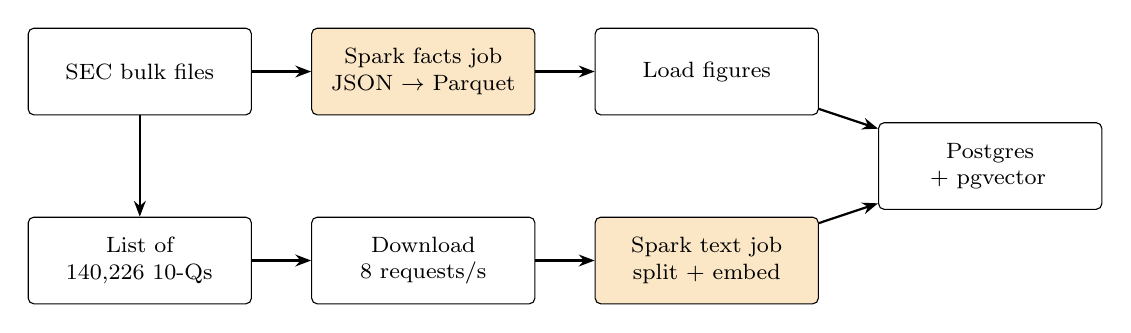
\begin{tikzpicture}[
  st/.style={draw,rounded corners=2pt,align=center,font=\footnotesize,text width=26mm,minimum height=11mm},
  sp/.style={st,fill=llmbox},
  arr/.style={-{Stealth[length=2mm]},thick}]
  \node[st] (fetch) at (0,0)     {SEC bulk files};
  \node[sp] (fj)    at (3.6,0)   {Spark facts job\\JSON $\to$ Parquet};
  \node[st] (lf)    at (7.2,0)   {Load figures};
  \node[st] (pg)    at (10.8,-1.2) {Postgres\\+ pgvector};
  \node[st] (man)   at (0,-2.4)  {List of\\140,226 10-Qs};
  \node[st] (dl)    at (3.6,-2.4) {Download\\8 requests/s};
  \node[sp] (tj)    at (7.2,-2.4) {Spark text job\\split + embed};
  \draw[arr] (fetch)--(fj); \draw[arr] (fj)--(lf); \draw[arr] (lf)--(pg);
  \draw[arr] (fetch)--(man); \draw[arr] (man)--(dl); \draw[arr] (dl)--(tj); \draw[arr] (tj)--(pg);
\end{tikzpicture}
\caption{The data pipeline. Shaded steps are Spark jobs. The text job processes downloaded documents
while later ones are still downloading.}
\label{fig:pipeline}
\end{figure}

\begin{table}[ht]
\centering\small
\begin{tabularx}{\linewidth}{Xr}
\toprule
Step & Time on c7i.8xlarge \\
\midrule
Download the SEC bulk files (\code{companyfacts.zip}, \code{submissions.zip}) & under 2 min \\
Spark facts job: 20,609 company files $\to$ Parquet & 40 s \\
Load the figures into Postgres & 60 s \\
List all 10-Qs since 2019 (140,226 filings) & 20 s \\
Download the 10-Qs at 8 requests/s, in 71 batches of 2,000 & about 5 h \\
Spark text job: split into passages, embed, load & about 8 h (overlaps the download) \\
\bottomrule
\end{tabularx}
\caption{Pipeline steps and their run time on the full data.}
\label{tab:pipeline}
\end{table}

The download of the 10-Qs stays just under the SEC's limit of 10 requests per second and stores each
document compressed. Computing embeddings is the most expensive step, so for most companies we keep
only the MD\&A section, which contains the explanations, rather than every section. This keeps about
30\% of the text. For the ten companies of our question set and the FinanceBench filings we keep
every section.

\subsection{Data processing with Spark}
\label{sec:spark}

Both batch jobs apply the same Python function to many independent input files and then combine the
results. Spark divides the files into partitions and processes them in parallel on all cores of the
machine.

\begin{figure}[ht]
\centering
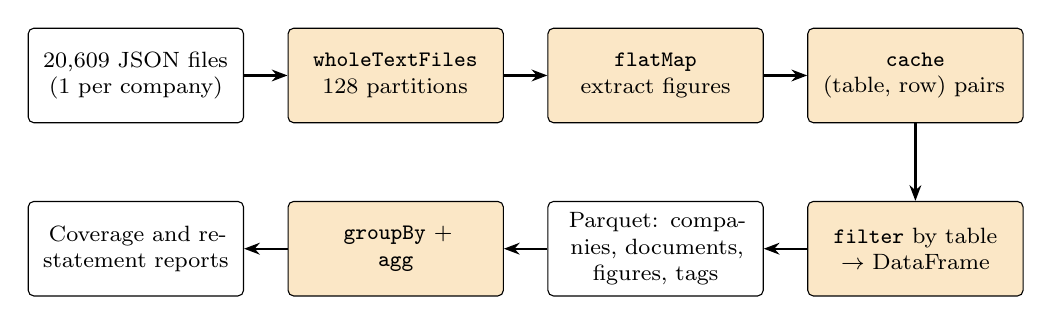
\begin{tikzpicture}[
  st/.style={draw,rounded corners=2pt,align=center,font=\footnotesize,text width=25mm,minimum height=12mm},
  sp/.style={st,fill=llmbox},
  arr/.style={-{Stealth[length=2mm]},thick}]
  \node[st] (in)  at (0,0)     {20,609 JSON files\\(1 per company)};
  \node[sp] (rd)  at (3.3,0)   {\code{wholeTextFiles}\\128 partitions};
  \node[sp] (fm)  at (6.6,0)   {\code{flatMap}\\extract figures};
  \node[sp] (ca)  at (9.9,0)   {\code{cache}\\(table, row) pairs};
  \node[sp] (fi)  at (9.9,-2.2) {\code{filter} by table\\$\to$ DataFrame};
  \node[st] (pq)  at (6.6,-2.2) {Parquet: companies, documents, figures, tags};
  \node[sp] (gb)  at (3.3,-2.2) {\code{groupBy} +\\\code{agg}};
  \node[st] (rep) at (0,-2.2)  {Coverage and restatement reports};
  \draw[arr] (in)--(rd); \draw[arr] (rd)--(fm); \draw[arr] (fm)--(ca); \draw[arr] (ca)--(fi);
  \draw[arr] (fi)--(pq); \draw[arr] (pq)--(gb); \draw[arr] (gb)--(rep);
\end{tikzpicture}
\caption{The Spark facts job. Shaded boxes are Spark operations; each partition is processed by one
core.}
\label{fig:spark}
\end{figure}

\paragraph{Facts job.} The job reads the 20,609 company files and splits them into 128 partitions,
four per core, so that every core stays busy although the files range from a few kilobytes to 30 MB.
A \code{flatMap} turns each file into rows for the four database tables. The result is kept in memory
(\code{cache}) because it is used once for each table, and each table is written as a Parquet file.
The job produces 9,695 companies, 140,436 10-Qs, 3,022,763 figures and 96,950 tag choices in 40
seconds. Two aggregations (\code{groupBy}) then report how many companies report each metric, and how
often a later filing reports a different value for the same quarter (62,483 cases). These
\emph{restatements} are why every figure keeps its filing.

\paragraph{Text job.} The text job reads the downloaded 10-Qs, splits every document into passages
and redistributes them evenly over the partitions, because documents differ greatly in length. Each
partition then embeds its passages in groups of 256, so the embedding model is loaded once per task
instead of once per passage.

\subsection{Updating with new filings}
\label{sec:update}

Companies file new 10-Qs every day. An update script runs the same pipeline on new data only: it adds
the figures of every filing newer than the newest one in the database and downloads and embeds only
the new documents. The facts job still reads all companies, because the SEC offers no file of recent
changes, but it takes under a minute.

\subsection{Deployment on AWS}

\Cref{tab:instance} shows the machine we used. Embedding millions of passages is CPU-bound and
parallel, so we chose a compute-optimised instance with many cores; E5 (\cref{sec:e5}) confirms that
the Spark jobs use up to its 16 physical cores. 64 GB of memory hold Spark and Postgres side by side,
and the 250 GB disk leaves ample room for the data in \cref{tab:storage}. After the full load the
same disk can be attached to a much smaller instance for serving, since answering a question needs
little computation.

\begin{table}[ht]
\centering\small
\begin{tabularx}{\linewidth}{lX}
\toprule
Setting & Value \\
\midrule
Instance type & c7i.8xlarge (compute-optimised): 32 vCPUs on 16 physical cores, 64 GB memory \\
Storage & 250 GB general-purpose SSD (gp3) \\
Operating system & Ubuntu, Docker Compose \\
Region & us-east-1 \\
Network access & SSH and the web page port from our own IP address only; database not exposed \\
Permissions & IAM role with access to our S3 bucket, so no keys are stored on the machine \\
\bottomrule
\end{tabularx}
\caption{EC2 instance.}
\label{tab:instance}
\end{table}

\begin{table}[ht]
\centering\small
\begin{tabularx}{\linewidth}{Xr}
\toprule
Data & Size \\
\midrule
\code{submissions.zip} & 1.5 GB \\
\code{companyfacts.zip}, unpacked into one JSON file per company & 19 GB \\
140,226 downloaded 10-Q documents & 17 GB \\
Passages with embeddings written by Spark (Parquet) & 8.7 GB \\
Postgres database & 12 GB \\
\quad of which passage embeddings (4.55 million $\times$ 384 numbers) & 6.7 GB \\
\quad of which passage text & 3.1 GB \\
\quad of which figures (3.0 million) and the other tables & 0.9 GB \\
Docker images (our image 2.6 GB, Postgres, Ollama with Qwen2.5-3B) and build cache & 22 GB \\
\midrule
Disk in use in total (\code{df}) & 77 GB of 242 GB \\
\bottomrule
\end{tabularx}
\caption{Data stored on the instance, measured with \code{du}, \code{docker system df} and Postgres'
\code{pg\_total\_relation\_size} after the full load and the update run. The database is smaller
than the raw files it was built from; the raw files and Parquet output could be moved to S3 after
loading.}
\label{tab:storage}
\end{table}

The FinanceBench PDFs were processed on a laptop and written into the cloud database through the SSH
tunnel, which the local Qwen models also used to reach the database during the experiments.

\section{Experiments}

We ran six experiments (\cref{tab:experiments}). E1 measures the quality of the answers, E2 the
search alone, and E3--E6 the cloud side.

\begin{table}[ht]
\centering\small
\begin{tabularx}{\linewidth}{llX}
\toprule
 & Experiment & What we measure \\
\midrule
E1 & Accuracy & Systems A, A0, A2, C and N with Haiku 5.5, Qwen2.5-7B and Qwen2.5-3B, on our question
              set and on FinanceBench: correct, wrong and declined answers, tokens and cost \\
E2 & Retrieval & BM25, semantic and hybrid search without an LLM \\
E3 & Latency per step & Time of each step, with Qwen2.5-3B on the CPU of the cloud machine \\
E4 & Load test & Questions per second and latency for 1, 10 and 50 users, without the LLM \\
E5 & Spark scaling & Run time of both Spark jobs with 1 to 32 cores \\
E6 & Updates & Time to add newly filed 10-Qs, measured and estimated for the busiest days \\
\bottomrule
\end{tabularx}
\caption{Experiments.}
\label{tab:experiments}
\end{table}

\subsection{Question sets}

\paragraph{Our question set.} We wrote 60 questions about ten large companies: 3M, Coca-Cola,
Johnson \& Johnson, Caterpillar and Honeywell (2023 filings), and PepsiCo, Tesla, Abbott, IBM and
Lockheed Martin (2024 filings). 50 form the test set; the other 10 are development questions, used
only to set the search threshold. The test set has six categories (\cref{tab:question-examples}),
including questions that the system should decline. Every correct answer was verified against the
filing itself, not against our database.

\begin{table}[ht]
\centering\small
\begin{tabularx}{\linewidth}{lrX}
\toprule
Category & $n$ & Example (correct answer) \\
\midrule
lookup     & 10 & ``What was 3M's revenue in Q2 2023?'' (\$8,325 million) \\
change     & 10 & ``How much did 3M's net sales change year over year in the second quarter of 2023?''
                  ($-4.3\%$, from \$8,702 million) \\
paraphrase & 8  & ``How big was J\&J's top line in Q1 2023?'' (revenue in everyday words) \\
why        & 12 & ``Why did Coca-Cola's operating income increase in Q2 2023?'' (favourable pricing
                  initiatives and channel and package mix) \\
decline    & 8  & ``What was IKEA's revenue in Q2 2024?'' (not an SEC filer: must be declined) \\
latest     & 2  & ``What was Honeywell's EPS?'' (no period: the latest quarter, with the assumption stated) \\
\bottomrule
\end{tabularx}
\caption{The six categories of our test set, with one example each.}
\label{tab:question-examples}
\end{table}

\paragraph{FinanceBench.} The 150 public FinanceBench questions~\cite{financebench}, written by
analysts about 84 filings, mostly annual reports. They come in three types of 50: calculations (``What
is Amazon's FY2017 days payable outstanding?''), questions that need an analyst's judgement (``Is 3M a
capital-intensive business based on FY2022 data?'') and other questions. As in the benchmark's
standard setting, every system is given the correct filing.

\subsection{Systems and models}

We run the workflow (A), its variants A0 (template answer) and A2 (with the financial statements),
simple RAG (C) and closed book (N). The hosted model is Claude Haiku 5.5. The local models are
Qwen2.5-7B and Qwen2.5-3B, run on a MacBook and connected to the cloud database; for E3, Qwen2.5-3B
also runs on the CPU of the cloud machine. To see how much a much larger model knows without any
documents, we also run N with Claude Opus 5.5. E3--E6 ran on the c7i.8xlarge. For E4 the LLM steps
are replaced by fixed outputs, so that only our own code is measured.

\subsection{Grading}
\label{sec:grading}

\paragraph{Numbers} are graded by code. An answer is correct if it states the correct value to the
precision it gives: ``\$8.3 billion'' is correct for \$8,325 million, ``\$8.4 billion'' is not. A
change must be within 0.15 percentage points.

\paragraph{Free text} (``why'' answers and all FinanceBench answers) is graded by an LLM judge
(Claude Haiku 5.5). It sees the question, the correct answer and the system's answer and decides
whether the answer is correct, incorrect or declined. To check the judge, a stronger model (Claude
Sonnet 5.5) graded a random sample of 300 of these answers again (\cref{tab:grader}). The two agree on
89\% of the answers, and on 95\% for the distinction that matters for accuracy, correct or not. Cohen's
$\kappa$, which corrects agreement for agreement by chance (1 is perfect, 0 is chance), is 0.84,
usually read as strong agreement.

\begin{table}[ht]
\centering\small
\begin{tabular}{lrrr}
\toprule
Judge (Haiku) $\downarrow$ \quad Sonnet $\rightarrow$ & correct & incorrect & declined \\
\midrule
correct   & \textbf{125} & 8  & 1 \\
incorrect & 4   & \textbf{74} & 18 \\
declined  & 1   & 0  & \textbf{69} \\
\bottomrule
\end{tabular}
\caption{Grader check on 300 random LLM-graded answers: verdicts of our judge (rows) against a
stronger model (columns).}
\label{tab:grader}
\end{table}

\subsection{Metrics}
\label{sec:metrics}

\begin{itemize}
  \item \textbf{Accuracy:} the share of questions answered correctly. A refusal counts as a decline:
        it is not correct, but it is reported separately from a \textbf{wrong answer}, because a
        wrong number is worse than none. \textbf{Wrong declines} are refusals of questions that could
        have been answered.
  \item \textbf{Repeated runs and confidence intervals.} Haiku gives slightly different answers each
        time, so every Haiku result was run three times and we report the mean $\pm$ the standard
        deviation. Qwen always gives the same answer, so it ran once. Because the test sets are
        small, we also report a 95\% confidence interval, computed by bootstrapping: we draw the
        questions with replacement 2,000 times and take the range that contains 95\% of the
        resulting accuracies.
  \item \textbf{Tokens and cost:} the number of text pieces (tokens) sent to and produced by the LLM per
        question, and the API cost per 1,000 questions.
  \item \textbf{Retrieval (E2):} \emph{hit@k} is the share of questions for which at least one correct
        passage is among the first $k$ search results. \emph{MRR} (mean reciprocal rank) averages
        $1/r$, where $r$ is the position of the first correct passage: 1 if it is first, 0.5 if
        second, 0 if it is not in the top 10.
  \item \textbf{Latency and throughput (E3, E4):} the median time per question (half of the questions
        are faster), the 95th percentile (95\% are faster), and the number of questions answered per
        second.
  \item \textbf{Speed-up (E5):} the run time on one core divided by the run time on $n$ cores; ideal
        scaling gives a speed-up of $n$.
\end{itemize}

\section{Results}

All numbers below come from the saved runs in \code{eval/results/} and are collected by
\code{eval/summarize.py} into \code{eval/RESULTS\_v2.md}. Haiku results are the mean $\pm$ standard
deviation over three runs; Qwen decodes greedily, so it has one run. The 95\% intervals come from a
bootstrap over the questions (\cref{sec:grading}).

\subsection{E1: accuracy on our question set}

\Cref{tab:e1-v2} and \cref{fig:e1-v2} show the accuracy on the 50 test questions. ``Wrong decl.''
counts questions the system refused although it should have answered (out of 42), ``Wrong'' the
answers that are simply wrong.

\begin{table}[ht]
\centering\small
\setlength{\tabcolsep}{3.5pt}
\resizebox{\linewidth}{!}{%
\begin{tabular}{llrrrrrr}
\toprule
System & Model & Accuracy \% & 95\% CI & Wrong decl. & Wrong & Tokens in / out & \$ / 1k q \\
\midrule
A workflow       & Haiku 5.5   & \textbf{96.0 $\pm$ 0.0} & 90--100 & 0.0 & 2.0 & 2,803 / 305 & 0.43 \\
A0 template      & Haiku 5.5   & 96.0 $\pm$ 0.0          & 90--100 & 0.3 & 1.7 & 2,384 / 204 & 0.34 \\
A2 workflow v2   & Haiku 5.5   & 96.0 $\pm$ 0.0          & 90--100 & 0.0 & 2.0 & 3,897 / 305 & 0.54 \\
C simple RAG     & Haiku 5.5   & 68.7 $\pm$ 1.2          & 56--82  & 0.3 & 15.3 & 3,583 / 462 & 0.59 \\
N closed book    & Haiku 5.5   & 30.7 $\pm$ 1.2          & 20--43  & 11.7 & 23.0 & 112 / 796  & 0.41 \\
N closed book    & Opus 5.5    & 62                      & 48--74  & 7   & 12   & 112 / 819  & 16.83 \\
\midrule
A workflow       & Qwen2.5-7B  & \textbf{84}  & 74--94 & 5  & 3  & 1,330 / 112 & 0 \\
A0 template      & Qwen2.5-7B  & 84           & 74--94 & 5  & 3  & 1,049 / 77  & 0 \\
C simple RAG     & Qwen2.5-7B  & 38           & 24--52 & 3  & 28 & 2,472 / 137 & 0 \\
N closed book    & Qwen2.5-7B  & 14           & 6--24  & 33 & 10 & 88 / 263    & 0 \\
\midrule
A workflow       & Qwen2.5-3B  & \textbf{62}  & 48--76 & 8  & 11 & 1,394 / 126 & 0 \\
A0 template      & Qwen2.5-3B  & 62           & 48--76 & 8  & 11 & 1,124 / 98  & 0 \\
C simple RAG     & Qwen2.5-3B  & 40           & 26--54 & 2  & 28 & 2,472 / 194 & 0 \\
N closed book    & Qwen2.5-3B  & 18           & 8--30  & 34 & 7  & 88 / 127    & 0 \\
\midrule
A workflow       & Qwen2.5-3B (EC2 CPU) & 54  & 40--66 & 14 & 9 & 1,052 / 131 & 0 \\
\bottomrule
\end{tabular}}
\caption{E1 on our question set (50 test questions). Haiku: mean $\pm$ standard deviation over three
runs (wrong declines and wrong answers are means); Qwen: one run. Tokens are the mean per question;
the last column is the cost per 1,000 questions. Local models cost nothing per question. The last
row runs Qwen2.5-3B with Ollama on the CPU of the EC2 instance.}
\label{tab:e1-v2}
\end{table}

\begin{figure}[ht]
\centering
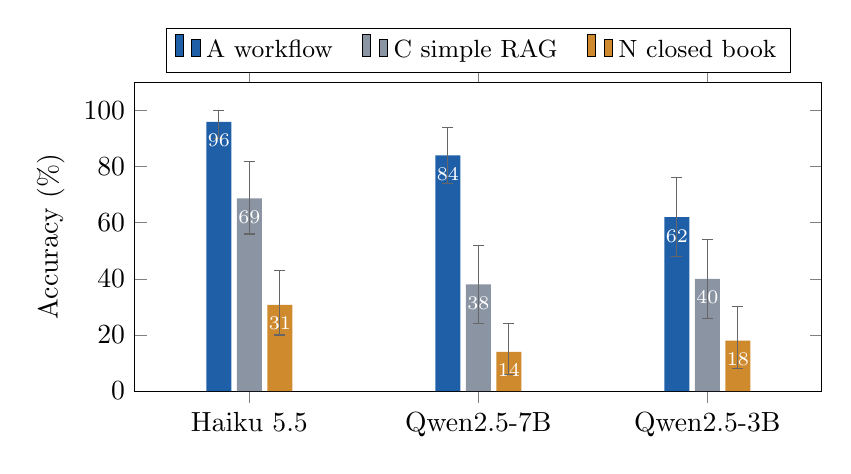
\begin{tikzpicture}
\begin{axis}[
  ybar, bar width=9pt, width=0.85\linewidth, height=55mm,
  ymin=0, ymax=110, ytick={0,20,40,60,80,100}, ylabel={Accuracy (\%)},
  symbolic x coords={Haiku 5.5,Qwen2.5-7B,Qwen2.5-3B}, xtick=data,
  enlarge x limits=0.25, legend style={at={(0.5,1.03)},anchor=south,legend columns=-1,font=\small,/tikz/every even column/.append style={column sep=3mm}},
  nodes near coords, every node near coord/.append style={/pgf/number format/precision=0, font=\scriptsize\bfseries, color=white, anchor=north, yshift=-1pt},
  error bars/y dir=both, error bars/y explicit, error bars/error bar style={black!60}]
\addplot[fill=wf,draw=none] coordinates {(Haiku 5.5,96) -= (0,6) += (0,4) (Qwen2.5-7B,84) -= (0,10) += (0,10) (Qwen2.5-3B,62) -= (0,14) += (0,14)};
\addplot[fill=rag,draw=none] coordinates {(Haiku 5.5,68.7) -= (0,12.7) += (0,13.3) (Qwen2.5-7B,38) -= (0,14) += (0,14) (Qwen2.5-3B,40) -= (0,14) += (0,14)};
\addplot[fill=cb,draw=none] coordinates {(Haiku 5.5,30.7) -= (0,10.7) += (0,12.3) (Qwen2.5-7B,14) -= (0,8) += (0,10) (Qwen2.5-3B,18) -= (0,10) += (0,12)};
\legend{A workflow, C simple RAG, N closed book}
\end{axis}
\end{tikzpicture}
\caption{E1 accuracy on our question set by system and model. The error bars are the 95\% bootstrap
intervals over the 50 questions.}
\label{fig:e1-v2}
\end{figure}

\Cref{tab:e1-cat} breaks the results down by category.

\begin{table}[ht]
\centering\small
\begin{tabular}{llrrrrrr}
\toprule
System & Model & Lookup & Change & Paraphrase & Why & Decline & Latest \\
 & & (10) & (10) & (8) & (12) & (8) & (2) \\
\midrule
A & Haiku 5.5  & 10 & 10 & 8 & 11 & 7 & 2 \\
C & Haiku 5.5  & 6  & 6  & 3 & 10.3 & 8 & 1 \\
N & Haiku 5.5  & 2.3 & 1.7 & 0 & 5.7 & 5.7 & 0 \\
\midrule
A & Qwen2.5-7B & 8  & 10 & 8 & 7  & 7 & 2 \\
C & Qwen2.5-7B & 1  & 0  & 1 & 8  & 8 & 1 \\
N & Qwen2.5-7B & 1  & 0  & 0 & 0  & 6 & 0 \\
\midrule
A & Qwen2.5-3B & 7  & 9  & 6 & 1  & 7 & 1 \\
C & Qwen2.5-3B & 2  & 1  & 2 & 7  & 8 & 0 \\
N & Qwen2.5-3B & 1  & 0  & 0 & 0  & 8 & 0 \\
\bottomrule
\end{tabular}
\caption{E1 correct answers per category on our question set (Haiku: mean of three runs; the
standard deviation is 0 except for C ``why'' (0.6) and N, where it is 0.6 to 1.5).}
\label{tab:e1-cat}
\end{table}

\paragraph{What the numbers show.}
\begin{itemize}
  \item \textbf{Numbers are where the workflow wins.} Simple RAG gets at most 6 of 10 changes right,
        because the statement tables are not in the 10-Q passages and the model only finds numbers
        that the text happens to mention. The workflow takes them from XBRL and computes the change
        in SQL, so even Qwen2.5-3B gets 9 of 10. The gap between A and C is larger than the
        confidence intervals for every model.
  \item \textbf{Small models gain the most.} With Qwen2.5-7B the workflow reaches 84\% against 38\%
        for simple RAG on the same passages. A model that runs on a laptop becomes useful once code
        does the numbers.
  \item \textbf{The workflow is stable across runs.} All three Haiku runs of A, A0 and A2 gave exactly
        the same 48 correct answers: the numbers come from SQL, so the model's randomness only
        affects the wording. Simple RAG and closed book vary by one to three answers between runs.
  \item \textbf{``Why'' questions are a draw for Haiku} (11 of 12 for A, 10.3 for C). For Qwen2.5-3B
        they are the weak spot of the workflow (1 of 12): its claims rarely pass the citation check,
        so the system declines instead of guessing.
  \item \textbf{Wrong declines come from small models misreading the question} (wrong company or
        metric): 5--8 of 42 for Qwen on the MacBook and 14 with the Ollama build of Qwen2.5-3B.
        Haiku had none with A.
  \item \textbf{Without retrieval the models mostly cannot answer.} The closed-book system N gets
        31\% with Haiku and 14--18\% with Qwen. Most of its answers say that the model does not know
        the figure, and the few numbers it gets right are hedged guesses (``around \$2 per share'')
        that cite no passage a reader could check. The much larger Opus 5.5 is different: without any
        retrieval it gets 62\% (one run), which we discuss in \cref{sec:contamination}.
  \item \textbf{Version 2 changes nothing here.} Our questions almost never reach document QA, so A2
        has the same accuracy as A, at about 1,100 more input tokens per question.
\end{itemize}

\paragraph{The answer writer (A vs.\ A0).} The writer LLM costs one to two seconds and a few hundred
tokens per answer. It never changed a number that reached the user: Haiku and Qwen2.5-7B passed the
check on every answer (38 of 38 and 36 of 36 in run 1), while Qwen2.5-3B failed it on 25 of 32
answers, mostly because it left out the references. Every rejected answer fell back to the template,
so A and A0 have the same accuracy for all models. The writer makes answers easier to read, but it is
not needed for correctness.

\subsection{E1: accuracy on FinanceBench}

\Cref{tab:e1-fb} shows FinanceBench. Unlike in the preliminary report, every model now answers all
150 questions.

\begin{table}[ht]
\centering\small
\setlength{\tabcolsep}{3.5pt}
\resizebox{\linewidth}{!}{%
\begin{tabular}{llrrrrrrrr}
\toprule
System & Model & Accuracy \% & 95\% CI & Wrong & Declined & Calc. & Analyst & Other & \$ / 1k q \\
\midrule
A workflow    & Haiku 5.5 & 69.1 $\pm$ 1.0 & 63--76 & 22.0 & 24.3 & 35.0 & 29.3 & 39.3 & 0.97 \\
A2 workflow v2 & Haiku 5.5 & \textbf{74.9 $\pm$ 1.0} & 68--81 & 24.3 & 13.3 & 42.3 & 31.3 & 38.7 & 1.19 \\
C simple RAG  & Haiku 5.5 & 54.4 $\pm$ 1.4 & 47--62 & 29.0 & 39.3 & 26.3 & 23.7 & 31.7 & 0.69 \\
N closed book & Haiku 5.5 & 21.3 $\pm$ 1.3 & 15--28 & 61.0 & 57.0 & 4.0  & 19.0 & 9.0  & 0.51 \\
N closed book & Opus 5.5  & 62.7           & 55--70 & 44   & 12   & 41   & 30   & 23   & 17.22 \\
\midrule
A workflow    & Qwen2.5-7B & 16.0 & 11--22 & 36 & 90 & 7  & 5  & 12 & 0 \\
C simple RAG  & Qwen2.5-7B & \textbf{23.3} & 17--31 & 64 & 51 & 10 & 12 & 13 & 0 \\
N closed book & Qwen2.5-7B & 8.0  & 4--13  & 112 & 26 & 0 & 8  & 4  & 0 \\
\midrule
A workflow    & Qwen2.5-3B & 14.7 & 9--21  & 69 & 59 & 4  & 5  & 13 & 0 \\
C simple RAG  & Qwen2.5-3B & \textbf{23.3} & 17--30 & 78 & 37 & 7  & 14 & 14 & 0 \\
N closed book & Qwen2.5-3B & 2.0  & 0--5   & 52 & 95 & 0  & 2  & 1  & 0 \\
\bottomrule
\end{tabular}}
\caption{E1 on FinanceBench (150 questions, 50 per type). Haiku: mean $\pm$ standard deviation over
three runs (counts are means); Opus and Qwen: one run. ``Calc.'' is metrics-generated, ``Analyst''
domain-relevant and ``Other'' novel-generated (correct answers out of 50 each).}
\label{tab:e1-fb}
\end{table}

\begin{itemize}
  \item \textbf{With Haiku the workflow is ahead of simple RAG in every question type,} and version 2
        adds another 5.8 points (69.1 to 74.9\%, with run-to-run deviations of 1.0). The gain is
        almost all on calculations (35.0 to 42.3 of 50), and it comes from fewer declines (24.3 to
        13.3), not from more guessing: the number of wrong answers stays about the same (22.0 and
        24.3). Code still evaluates every formula from cited inputs; only 3 of 900 workflow answers
        used an input that was not printed in a retrieved passage, and all three were flagged.
  \item \textbf{With small models the result flips.} Qwen2.5-7B gets 16\% with the workflow and 23\%
        with simple RAG. Document QA asks the model for structured output: an answer, cited claims
        and, for calculations, each input with its passage and a formula. Qwen often cannot produce
        this from long 10-K passages, so the system declines (90 of 150) instead of guessing. It
        gives far fewer wrong answers than simple RAG (36 against 64), but also fewer right ones.
  \item \textbf{Without retrieval, Haiku and Qwen mostly fail,} and they fail badly: closed-book Haiku
        gives 61 wrong answers, more than any system with retrieval, and Qwen2.5-7B answers almost
        everything from memory and gets 112 of 150 wrong. A small model that guesses from memory is
        the most dangerous setup for financial data.
  \item \textbf{Opus 5.5 without any filing gets 62.7\%,} close to our workflow with Haiku, and 41 of
        50 calculations. We discuss what this means in \cref{sec:contamination}.
\end{itemize}

\subsection{Why version 2 helps: FinanceBench error analysis}
\label{sec:fb-errors}

After the first run we read all 46 answers of version 1 (Haiku, run 1) that were wrong or declined,
together with the gold answer and its evidence page, and assigned each to one cause. Only then did we
build version 2, and we ran it once on all questions without further changes. \Cref{tab:fb-errors}
lists the causes and what version 2 does with the same questions (majority verdict of its three
runs).

\begin{table}[ht]
\centering\small
\begin{tabularx}{\linewidth}{Xrrrr}
\toprule
Cause of the v1 failure & $n$ & v2 correct & v2 wrong & v2 declined \\
\midrule
A financial statement was needed but not retrieved & 14 & \textbf{11} & 3 & 0 \\
Another page was not retrieved (cover page, debt table, earnings release) & 9 & 2 & 0 & 7 \\
Different definition than the gold answer (quick ratio, working capital, capital intensity) & 9 & 1 & 8 & 0 \\
Wrong reasoning or conclusion (including one sign error) & 5 & 2 & 3 & 0 \\
Metric not meaningful for the company (bank, card issuer) & 2 & 1 & 0 & 1 \\
Rounding, or a strict grade (\$8.74 billion for \$8.70 billion) & 2 & 0 & 2 & 0 \\
Wrong line item or scope (segment instead of company) & 2 & 0 & 2 & 0 \\
Incomplete list (acquisitions, regions) & 2 & 1 & 1 & 0 \\
Formula could not be evaluated & 1 & 0 & 0 & 1 \\
\midrule
Total & 46 & 18 & 19 & 9 \\
\bottomrule
\end{tabularx}
\caption{Causes of the 46 wrong or declined answers of version 1 (Haiku, run 1), and the verdict of
version 2 on the same questions (majority verdict of its three runs).}
\label{tab:fb-errors}
\end{table}

\paragraph{What the analysis shows.} Half of the declines (14 of 26) had the same cause: the
calculation needed a line of the balance sheet, income statement or cash-flow statement, and the
search did not return that page. Version 2 fixes 11 of these 14. Over all 150 questions (majority of
three runs), 11 declines and 4 wrong answers of version 1 become correct, while 5 correct answers get
worse, so the net gain is 10 questions. The remaining failures need different fixes:
\begin{itemize}
  \item \textbf{Definitions.} Nine ``wrong'' answers computed a reasonable but different metric, for
        example the quick ratio as (cash + receivables) / current liabilities instead of the gold
        answer's (current assets $-$ inventory) / current liabilities. These are differences of
        convention rather than reading errors; stating the definition in the answer, which the
        workflow does, lets a reader see it.
  \item \textbf{Pages outside the statements.} Questions about the cover page (``Which debt securities
        are registered\ldots''), a debt maturity table or an earnings release still fail because
        search does not find the page; v2 mostly declines them, which is the right behaviour when the
        evidence is missing.
  \item \textbf{Judgement.} Questions such as ``Is 3M a capital-intensive business?'' have no single
        right number. The workflow answers with one metric and the gold answer uses another.
\end{itemize}
Because version 2 was motivated by failures on FinanceBench itself, its FinanceBench score is
somewhat optimistic. We limited this by making one general change, choosing it before running it, and
not tuning anything after the run; the same change makes no difference on our own question set,
where the statements are already covered by SQL.

\subsection{Is FinanceBench in the training data?}
\label{sec:contamination}

Closed-book Haiku gets 21\% of FinanceBench, but closed-book Opus 5.5 gets 62.7\%, including 41 of 50
calculations such as ``What is the FY2018 capital expenditure amount for 3M?'' without seeing the
filing. There are two possible reasons: Opus has memorised the figures of these well-known companies'
10-Ks, or it has seen FinanceBench itself, which has been public since 2023 with its answers.
To tell these apart, we also ran closed-book Opus on our own question set, which did not exist
before this project. It gets 62\% there as well (31 of 50, 95\% interval 48--74), for example 3M's Q2
2023 net sales of \$8,325 million and Tesla's gross profit for Q3 2024, both from memory. It cannot
answer for the latest quarter (Q3 2026), which came after its training data: it lists older quarters
instead and says it does not know whether newer ones exist. So Opus has not simply memorised
FinanceBench. It has memorised the reported figures of large US companies up to its training cut-off,
which our ten companies and FinanceBench's 40 have in common. Its answers are still not usable as they
are: they are marked from memory'', cite no passage, and 12 of the 50 are wrong.

This has two consequences. First, any benchmark built from the filings of large companies before a
model's cut-off, ours included, cannot show on its own whether a large model reads the document or
remembers the answer; a closed-book run of the same model is the baseline that retrieval has to beat.
Second, the value of retrieval for a strong model is less in the score than in what it adds to it:
answers about filings after the cut-off (new quarters, and the thousands of smaller companies in the database),
and a citation to the exact passage or XBRL fact, so that a reader can check every number.

\subsection{Examples}
\label{sec:examples}

\paragraph{Retrieval.} \Cref{tab:retrieval-example} shows the top three passages of each search
method for two ``why'' questions, searched in the MD\&A of the correct 10-Q. For Coca-Cola all three
hybrid results contain the gold reasons (``favorable pricing initiatives'', ``favorable channel and
package mix''); BM25 and semantic search each put a less useful passage first. Searching the whole
filing instead of the MD\&A makes semantic search worse: its top three are the accounting-policy note,
the exhibit index and the equity table, which are about ``Coca-Cola'' and ``Q2 2023'' in general. For
3M no method finds the reasons in the top three: the evidence (``disposable respirator sales
decline'') sits in the segment discussion, while the top results are the general overview, which
uses the question's words (``sales'', ``second quarter'') more often. The workflow then gives the
figures but only part of the explanation, which is what happened in E1.

\begin{table}[ht]
\centering\small
\begin{tabularx}{\linewidth}{llX}
\toprule
Method & Hits & Top three passages (section › heading) \\
\midrule
\multicolumn{3}{l}{\emph{``Why did Coca-Cola's operating income increase in Q2 2023?''}} \\
BM25     & 2 of 3 & Equity income (miss); Operating income: Global Ventures (hit); Operating income: Latin America (hit) \\
Semantic & 2 of 3 & Unit case volume (miss); Operating income: Asia Pacific (hit); Global Ventures (hit) \\
Hybrid   & 3 of 3 & Operating income: Global Ventures, Latin America, Asia Pacific (all hits) \\
\midrule
\multicolumn{3}{l}{\emph{``Why did 3M's sales drop in Q2 2023?''}} \\
BM25     & 0 of 3 & Overview: financial condition; Results of operations: ERP system; Overview \\
Semantic & 0 of 3 & Overview; Overview: financial condition; Financial condition and liquidity \\
Hybrid   & 0 of 3 & Overview: financial condition; Overview; Results of operations \\
\bottomrule
\end{tabularx}
\caption{Real search results for two ``why'' questions (MD\&A only). A hit contains one of the
question's evidence phrases.}
\label{tab:retrieval-example}
\end{table}

\paragraph{Declines.} \Cref{tab:decline-examples} shows how the workflow (Haiku) answered the decline
questions. Each refusal names its reason, which comes from code, not from the LLM: the company is not
in the database, the period would need a 10-K, the company does not report the metric in its XBRL
data, or the passages do not contain the answer. The one ``failure'' is instructive: we expected the
system to decline Coca-Cola's gross margin because margins are not one of our ten metrics, but
document QA found the sentence ``gross profit margin increased to 59.0 percent'' in the 10-Q and
answered correctly with a citation. Our answer key was stricter than necessary here. The closed-book
system, in contrast, answered two decline questions from memory, for example a figure that is only in
a 10-K.

\begin{table}[ht]
\centering\small
\begin{tabularx}{\linewidth}{XX}
\toprule
Question & Answer of the workflow (status) \\
\midrule
What was IKEA's revenue in Q2 2024? & Not enough evidence: no filings for `IKEA' are loaded.
  (abstain) \\
What was Johnson \& Johnson's Q4 2023 revenue? & No filing of Johnson \& Johnson for Q4 2023 is
  loaded (Q4 data is not reported in 10-Q filings). (abstain) \\
What was 3M's R\&D expense in Q2 2023? & 3M does not report research \& development expense in its
  10-Q data (none of the XBRL tags \ldots\ is reported). (abstain) \\
Why did 3M's stock price fall after the earnings release? & The filing passages do not answer this
  question. (abstain) \\
What was Coca-Cola's gross margin percentage in Q2 2023? & Gross profit margin was 59.00 percent
  [C321889]. (answered; expected a decline) \\
\bottomrule
\end{tabularx}
\caption{Answers of the workflow to decline questions of our test set (Haiku 5.5).}
\label{tab:decline-examples}
\end{table}

\subsection{E2: retrieval}

\Cref{tab:e2} compares the three search methods without any LLM. For our ``why'' questions a hit is
a passage that contains one of the evidence phrases; for FinanceBench it is a passage from the
evidence page. MRR is the mean reciprocal rank of the first hit in the top 10.

\begin{table}[ht]
\centering\small
\begin{tabular}{lrrrrrrr}
\toprule
 & \multicolumn{3}{c}{``Why'' questions, MD\&A (12)} & \multicolumn{3}{c}{FinanceBench (150)} & \\
\cmidrule(lr){2-4}\cmidrule(lr){5-7}
Method & hit@1 & hit@5 & MRR & hit@1 & hit@10 & MRR & ms \\
\midrule
BM25            & 0.25 & 0.83 & 0.49 & 0.19 & 0.45 & 0.26 & 9--50 \\
Semantic (MiniLM) & 0.33 & 0.75 & 0.53 & 0.26 & 0.65 & 0.36 & 12--25 \\
Hybrid (RRF)    & \textbf{0.50} & 0.83 & \textbf{0.61} & \textbf{0.29} & 0.65 & \textbf{0.40} & 9--47 \\
\bottomrule
\end{tabular}
\caption{E2 retrieval quality and median search time. Search is deterministic, so there is one run;
with 12 questions one question changes hit@1 by 0.08.}
\label{tab:e2}
\end{table}

Hybrid search puts the right passage first twice as often as BM25 on ``why'' questions and has the
best MRR on both sets, at the same speed, so it is the default. The development questions set the
evidence threshold to a cosine similarity of 0.45: the lowest top score of a development search that
found its evidence was 0.464, and our first guess of 0.55 would have declined 3 of 8 answerable
questions. FinanceBench is harder for search (hit@10 of 0.65) because its evidence is often a table
in a 100-page 10-K, which is exactly the gap that version 2 closes by giving the statements directly.
With only 12 ``why'' questions the differences between the methods are small in absolute terms (one
question is 0.08), so we read E2 as ``hybrid is at least as good as either method alone'' rather than
as a precise ranking.

\subsection{E3: latency per step}

\begin{table}[ht]
\centering\small
\begin{tabular}{lrr}
\toprule
Step & Number question (ms) & ``Why'' question (ms) \\
\midrule
LLM parse & 4,301 & 4,341 \\
SQL: company / filing / figures & 1.3 / 0.7 / 1.1 & 1.7 / 0.6 / 2.9 \\
Question embedding / vector search / ranking & -- & 2.9 / 3.0 / 0.0 \\
LLM claims & -- & 15,439 \\
LLM writer & 2,940 & 5,838 \\
\midrule
Total (median) & 7,072 & 25,726 \\
\bottomrule
\end{tabular}
\caption{E3 median time per step on the c7i.8xlarge, with Qwen2.5-3B on the CPU (Ollama), over the
answered questions of one run (18 number and 11 ``why'' questions).}
\label{tab:e3}
\end{table}

Our own steps (SQL and search) take less than 10 ms per question. Everything else is LLM time: an LLM
call takes 100 to 1,000 times longer than the rest of the pipeline. Running Qwen2.5-3B on the CPU of
the instance works without any API key, but it is slower and less accurate (54\%) than the same
model on a laptop's Apple GPU (62\%, 9 s per question including the SSH tunnel).

\subsection{E4: load test}
\label{sec:e4}

\paragraph{The pipeline in one process.} With the LLM steps replaced by fixed outputs, only SQL,
search and code run (\cref{tab:e4}).

\begin{table}[ht]
\centering\small
\begin{tabular}{rrrr}
\toprule
Concurrent users & Questions / s & Median ms & p95 ms \\
\midrule
1  & 82.8  & 11  & 17 \\
10 & 284.5 & 34  & 46 \\
50 & 221.5 & 206 & 322 \\
\bottomrule
\end{tabular}
\caption{E4 throughput and latency of one Python process on the c7i.8xlarge, without the LLM
(30 seconds per step).}
\label{tab:e4}
\end{table}

One Python process serves about 280 questions per second at 10 users. At 50 users it is saturated
and latency grows, because one Python process runs Python code on one core at a time; more worker
processes, or several instances behind a load balancer, are the next step.

\paragraph{The HTTP API on three instance sizes.} The second part of E4 tests the deployed API with
up to 1,000 users on c7i.large, c7i.xlarge and c7i.2xlarge (\cref{sec:experiments-e4}). Two changes
were needed before it could work at all. A request used to open its database connection before the
LLM parse step, so 1,000 requests waiting for an LLM would have held 1,000 connections, ten times
Postgres' default limit of 100; the connection is now opened after the parse, and the limit is
raised to 500. And FastAPI serves synchronous requests from a pool of 40 threads per process, which
would cap the number of requests waiting for an LLM at the same time; the test server raises it.

\resultsplaceholder{E4 HTTP results: answers per second, median / p95 / p99 latency and error rate
for 1--1,000 users on c7i.large, c7i.xlarge and c7i.2xlarge, with no LLM wait and with a 5-second
LLM wait. To be run once the AWS vCPU quota allows the three extra instances.}

\subsection{E5: Spark scaling}
\label{sec:e5}

\begin{figure}[ht]
\centering
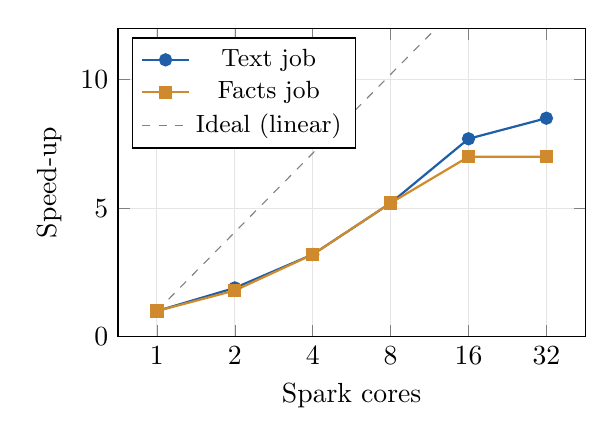
\begin{tikzpicture}
\begin{axis}[
  width=0.62\linewidth, height=55mm, xmode=log, log basis x=2,
  xtick={1,2,4,8,16,32}, xticklabels={1,2,4,8,16,32},
  xlabel={Spark cores}, ylabel={Speed-up}, ymin=0, ymax=12,
  legend pos=north west, legend style={font=\small}, grid=major, grid style={gray!20}]
\addplot[wf,thick,mark=*] coordinates {(1,1.0) (2,1.9) (4,3.2) (8,5.2) (16,7.7) (32,8.5)};
\addplot[cb,thick,mark=square*] coordinates {(1,1.0) (2,1.8) (4,3.2) (8,5.2) (16,7.0) (32,7.0)};
\addplot[gray,dashed,domain=1:12,samples=2] {x};
\legend{Text job, Facts job, Ideal (linear)}
\end{axis}
\end{tikzpicture}
\hspace{4mm}
\begin{minipage}[b]{0.3\linewidth}\small
\begin{tabular}{rrr}
\toprule
Cores & Text s & Facts s \\
\midrule
1 & 170 & 284.8 \\
2 & 90 & 157.3 \\
4 & 53 & 88.3 \\
8 & 33 & 55.0 \\
16 & 22 & 40.6 \\
32 & 20 & 40.6 \\
\bottomrule
\end{tabular}
\vspace{6mm}
\end{minipage}
\caption{E5 speed-up of the two Spark jobs on one c7i.8xlarge (32 vCPUs = 16 physical cores with
two threads each). The text job ran on 80 filings (2,458 passages), the facts job on all 20,609
company files; one run per core count.}
\label{fig:e5}
\end{figure}

Both jobs scale well up to 8 cores (5.2 times faster) and still gain up to 16. Going from 16 to 32
adds little, for two reasons: the 32 vCPUs are only 16 physical cores, and Spark's fixed start-up
time weighs more on these small test jobs. On the full batches of 2,000 filings the instance reached
130 to 190 passages per second.

\subsection{E6: updates with new filings}
\label{sec:e6}

\Cref{tab:e6} shows the update run of 26 November 2026. Since the last load (filings up to 20
November) the SEC had received 92 new 10-Qs, including three companies that were not in the database
yet. The whole update took five minutes. 53 of the 92 filings had an MD\&A section that our splitter
recognised; they gave 1,950 new passages. (The share is the same as in the full run, where 72\% of
the 10-Qs got text.)

\begin{table}[ht]
\centering\small
\begin{tabularx}{\linewidth}{Xr}
\toprule
Step (c7i.8xlarge, 32 vCPUs) & Seconds \\
\midrule
1. Download the SEC bulk files again (\code{companyfacts.zip}, \code{submissions.zip}, 2.8 GB) & 114 \\
2. Spark facts job on all 20,609 companies (38 s inside Spark; the rest is starting the container and Spark) & 124 \\
3. Load facts: 92 new filings, 3 new companies, 2,744 new figures & 17 \\
4. Manifest of the new filings & 7 \\
5. Download the 92 10-Qs & 13 \\
6. Spark text job: split and embed (1,950 passages) & 25 \\
7. Load the passages & 2 \\
\midrule
Total & 301 \\
\bottomrule
\end{tabularx}
\caption{E6: one update run, adding the 10-Qs filed from 21 to 26 November 2026.}
\label{tab:e6}
\end{table}

\paragraph{How much does a busy day need?} Late November is a quiet time. \Cref{fig:filings-per-day}
shows how many 10-Qs the SEC receives per day: about 17,500 a year, but very unevenly. On a median
day there are only 16, while in the two weeks after each quarter's deadline there are several hundred
per day, with a maximum of 718 (7 November 2024). For the busiest day we can estimate the update time
from the measured rates. The download is limited by the SEC to under 10 requests per second, so 718
filings take about 90 seconds on any instance. At about 37 passages per filing, they give about
26,600 passages to embed: about 3 minutes at the 130--190 passages per second of the c7i.8xlarge,
or about 16 minutes on a c7i.large with 2 vCPUs (27 passages per second in E5). Adding the bulk
download and the facts job (2 to 3 minutes), even the busiest day of the year is updated in under
10 minutes on the large instance and in about 25 minutes on the smallest one. A daily update
therefore does not need the large instance at all: a small instance that runs once a night is enough,
and the large one is only needed for the first full load, which processed the 140,000 10-Qs of seven
years in about 9 hours.

\begin{figure}[ht]
\centering
\begin{tikzpicture}
\begin{axis}[
  width=0.95\linewidth, height=45mm, ybar interval, ymode=log, log origin=infty, ymin=0.8, ymax=1000,
  xlabel={10-Qs filed on one day}, ylabel={Days (2024--2026)},
  xmin=0, xmax=800, enlarge x limits=false, x tick label as interval=false,
  xtick={0,100,200,300,400,500,600,700,800}, xticklabel style={font=\footnotesize},
  yticklabel style={font=\footnotesize}, grid=major, grid style={gray!20}]
\addplot[fill=wf,draw=white] table[x=bin,y=days] {figures/filings_hist.dat};
\end{axis}
\end{tikzpicture}
\caption{E6: how many 10-Qs the SEC receives per day, from \code{submissions.zip} (2024 to November
2026, 720 working days). Most days have under 50; about 20 days a year have over 300.}
\label{fig:filings-per-day}
\end{figure}

\section{Conclusion}

We built a question-answering agent over SEC filings in which the LLM only reads the question and
phrases the answer, while SQL, search and code find every number, compute every change and check
every citation. On AWS, a Spark pipeline on one EC2 instance loaded the figures and 10-Q text of
every SEC filer since 2019: 9,695 companies, 140,436 10-Qs, 3.0 million figures and 4.55 million
passages, for about \$20. An update run adds each day's new filings in minutes.

The experiments show four things. First, the workflow is much more accurate than simple RAG on
quarterly numbers (96\% against 69\% with Claude Haiku 5.5, identical over three runs), and the gap
is largest for small local models (84\% against 38\% with Qwen2.5-7B on a laptop). Second, on the
external FinanceBench benchmark the workflow is ahead of simple RAG in every question type with Haiku
(69\% against 54\%), and version 2, which always gives the model the three financial statements,
raises this to 75\% by turning declines into correct answers, with about as many wrong answers as
before. Its
structured answer format is still too demanding for small models. Third, a closed-book baseline shows
that retrieval is needed: without it Haiku answers 31\% of our questions and 21\% of FinanceBench, with
no source a reader can check. The much larger Opus 5.5, however, answers 63\% of FinanceBench and
62\% of our questions without any filing: it remembers the figures of large companies, so scores on
filings from before a model's cut-off must be compared with a closed-book baseline, and the value of
retrieval lies in newer filings, smaller companies and checkable citations. Fourth, our own layer is fast (about 10 ms per question, more than 200 questions
per second in one process), the Spark jobs scale to the physical cores of the machine, and even the
busiest filing day of the year can, by our estimate from the measured rates, be added in under half
an hour on the smallest instance. The LLM
and the SEC download limit are the only real bottlenecks.

\paragraph{Limitations.} About 27\% of 10-Qs have no MD\&A heading that our section detector
recognises, so they have no text. Quarters are calendar quarters, so for companies with a different
fiscal year ``Q2'' means April to June. Passages from 10-Q HTML leave out tables, so ratio questions
on bulk 10-Qs usually decline. Document QA checks that the inputs of a calculation are printed in the
filing, but not that they are the right lines, and analysts' metrics such as the quick ratio have
several definitions. Version 2 was motivated by FinanceBench failures, so its FinanceBench score is
somewhat optimistic. Free-text grades come from an LLM judge that agrees with a stronger model on 89\% of
a sample of 300 ($\kappa = 0.84$); a check by a person is still to do.

\paragraph{Next steps.} Before the final report we plan to (1) check the grader sample by hand,
(2) run the HTTP load test with up to 1,000 users on three instance sizes, (3) give small models a
simpler document QA format, and (4) improve the MD\&A detector and keep tables in 10-Q passages.


\clearpage
\bibliographystyle{IEEEtran}
\bibliography{references}

\section*{AI declaration}
\addcontentsline{toc}{section}{AI declaration}

We used AI tools (Claude Code) in this project for the following purposes:
\begin{enumerate}
  \item to help write and debug code, tests and deployment scripts;
  \item to help write the README, the reproduction guide and this report, and to improve their
        clarity and grammar.
\end{enumerate}
The LLMs that are part of the system (Claude Haiku 5.5, Qwen2.5) and the LLM grader are described in
the report itself. The project idea, the design decisions and the evaluation are our own, and we
checked all reported numbers against the saved experiment results.


\end{document}
